\documentclass[border=3pt]{standalone}
\usepackage{fontspec}
\usepackage{unicode-math}
\setmainfont{TeX Gyre Heros}
\setmathfont{TeX Gyre Termes Math}
\usepackage{tikz}
\usetikzlibrary{arrows.meta,calc}
\definecolor{pass}{HTML}{1F4E79}
\definecolor{passfill}{HTML}{EAF1F8}
\definecolor{block}{HTML}{6E6E6E}
\definecolor{blockfill}{HTML}{F0F0F0}
\definecolor{ink}{HTML}{222222}
\begin{document}
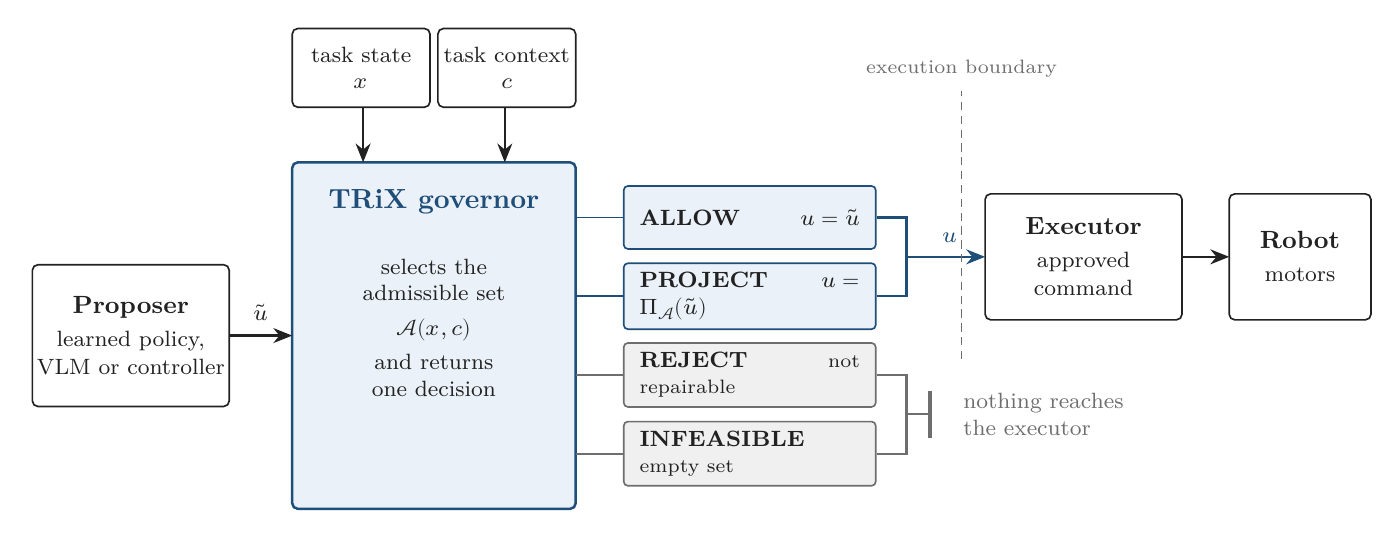
\begin{tikzpicture}[x=1mm, y=1mm, font=\small, ink,
  >={Stealth[length=2.4mm,width=1.9mm]},
  flow/.style={->, line width=0.8pt},
  lab/.style={font=\footnotesize, align=center},
  chip/.style={rounded corners=1.5pt, line width=0.6pt, minimum height=8mm,
               text width=28mm, inner xsep=2mm, font=\footnotesize, anchor=west}]

% proposer
\draw[line width=0.6pt, rounded corners=2pt] (0,-9) rectangle (25,9);
\node[align=center] at (12.5,0) {\textbf{Proposer}\\[1pt]{\footnotesize learned policy,}\\[-1pt]{\footnotesize VLM or controller}};

% governor
\draw[line width=0.9pt, draw=pass, fill=passfill, rounded corners=2pt] (33,-22) rectangle (69,22);
\node[font=\normalsize\bfseries, text=pass] at (51,17) {TRiX governor};
\node[lab] at (51,1) {selects the\\admissible set\\[3pt] $\mathcal{A}(x,c)$\\[3pt] and returns\\one decision};

% inputs
\draw[line width=0.6pt, rounded corners=2pt] (33,29) rectangle (50.5,39);
\node[lab] at (41.75,34) {task state\\$x$};
\draw[line width=0.6pt, rounded corners=2pt] (51.5,29) rectangle (69,39);
\node[lab] at (60.25,34) {task context\\$c$};
\draw[flow] (42,29) -- (42,22);
\draw[flow] (60,29) -- (60,22);

% proposal
\draw[flow] (25,0) -- (33,0);
\node[lab, anchor=south] at (29,0.6) {$\tilde u$};

% decisions
\node[chip, fill=passfill, draw=pass] (allow) at (75,15)
  {\textbf{ALLOW}\hfill $u=\tilde u$};
\node[chip, fill=passfill, draw=pass] (project) at (75,5)
  {\textbf{PROJECT}\hfill $u=\Pi_{\mathcal{A}}(\tilde u)$};
\node[chip, fill=blockfill, draw=block] (reject) at (75,-5)
  {\textbf{REJECT}\hfill {\scriptsize not repairable}};
\node[chip, fill=blockfill, draw=block] (infeas) at (75,-15)
  {\textbf{INFEASIBLE}\hfill {\scriptsize empty set}};
\foreach \y in {15,5} \draw[line width=0.7pt, pass] (69,\y) -- (75,\y);
\foreach \y in {-5,-15} \draw[line width=0.7pt, block] (69,\y) -- (75,\y);

% forwarded path
\draw[line width=0.8pt, pass] (allow.east) -| (111,10);
\draw[line width=0.8pt, pass] (project.east) -| (111,10);
\draw[flow, pass] (111,10) -- (121,10);
\node[lab, text=pass, anchor=south] at (116.5,10.6) {$u$};

% blocked path
\draw[line width=0.8pt, block] (reject.east) -| (111,-10);
\draw[line width=0.8pt, block] (infeas.east) -| (111,-10);
\draw[line width=0.8pt, block] (111,-10) -- (114,-10);
\draw[line width=1.6pt, block] (114,-13) -- (114,-7);
\node[lab, text=block, anchor=west, align=left] at (117,-10) {nothing reaches\\the executor};

% boundary
\draw[densely dashed, line width=0.5pt, block] (118,-3) -- (118,31);
\node[font=\scriptsize, text=block, anchor=south] at (118,31.5) {execution boundary};

% executor and robot
\draw[line width=0.6pt, rounded corners=2pt] (121,2) rectangle (146,18);
\node[align=center] at (133.5,10) {\textbf{Executor}\\[1pt]{\footnotesize approved}\\[-1pt]{\footnotesize command}};
\draw[line width=0.6pt, rounded corners=2pt] (152,2) rectangle (170,18);
\node[align=center] at (161,10) {\textbf{Robot}\\[1pt]{\footnotesize motors}};
\draw[flow] (146,10) -- (152,10);

\end{tikzpicture}
\end{document}
